\documentclass[a4paper, 12pt]{article}%тип документа

%отступы
\usepackage[left=1.5cm,right=1cm,top=2cm,bottom=3cm,bindingoffset=0cm]{geometry}
\setlength{\parindent}{5ex}

%Русский язык
\usepackage[T2A]{fontenc} %кодировка
\usepackage[utf8]{inputenc} %кодировка исходного кода
\usepackage[english,russian]{babel} %локализация и переносы

%Вставка картинок
\usepackage{graphicx}
\graphicspath{{pictures/}}
\DeclareGraphicsExtensions{.pdf,.png,.jpg,}
\usepackage{wrapfig}

%Графики
\usepackage{pgfplots}
\pgfplotsset{compat=1.9}

%Математика
\usepackage{amsmath, amsfonts, amssymb, amsthm, mathtools}

%Таблицы
\usepackage{longtable} 

%Римские цифры
\newcommand{\RomanNumeralCaps}[1]{\uppercase\expandafter{\romannumeral#1}}

\usepackage{multirow}
\usepackage{floatrow}


\begin{document}
	\begin{titlepage}
		\begin{center}
			\textsc{Федеральное государственное автономное образовательное учреждение высшего образования«Московский физико-технический институт (национальный исследовательский университет)»\\[5mm]
			}
			
			\vfill
			
			\textbf{Вопрос по выбору: \\[3mm]
				Эффект Зеемана
				\\[50mm]
			}
			
		\end{center}
		
		\hfill
		\begin{minipage}{.5\textwidth}
			Выполнили студенты:\\[2mm]
			Сериков Василий Романович\\[2mm]
			Группа: Б03-102\\[5mm]
			Сериков Алексей Романович\\[2mm]
			Группа: Б03-102\\[5mm]
			
		\end{minipage}
		\vfill
		\begin{center}
			Москва, 2024 г.
		\end{center}
		
	\end{titlepage}
	
	\newpage
	\textbf{Аннотация}\\
	
	Цель работы состоит в изучении интерферометра и эталона Фабри-Перо. Также исследуется поведение атомных линий в поперечном магнитном поле при расщеплении линий ртути (Эффект Зеемана)\\
	
	
	\textbf{Теоретические сведения: }\\
	
	\textbf{Классическая интерпретация эффекта Зеемана: }\\
	
	Теория явления, предложенная Лоренцом в 1897 г., основана на представлениях классической электродинамики. В соответствии с этими представлениями, линейчатое излучение атома обусловлено движением электронов в атоме по простому гармоническому закону. Магнитное поле воздействует на движущийся заряд, замедляя или ускоряя его в зависимости от знака заряда и взаимного направления скорости заряда и магнитного поля (сила Лоренца).
	
	Любое гармоническое колебание электрона в отсутствие поля можно разложить на три составляющих: одно колебание вдоль поля и два круговых движения по кругу - левое и правое, которые происходят в плоскости, перпендикулярной полю. В результате мы получим, что при включении поля колебание вдоль направления поля не изменит свою частоту. В то же время в круговом движении появится добавочная сила, которая в одном направлении ускорит вращение, а в другом - замедлит. Соответственно, и в излучении атома, помещенного в магнитное поле, появятся три спектральные линии. Одна из этих линий, так называемая $\pi$ компонента, совпадает по частоте с линией, излучаемой свободным атомом, и поляризована линейно в направлении магнитного поля. Две другие, так называемые $\sigma$-компоненты, соответствующие круговым движениям, оказываются смещенными по частоте симметрично относительно центральной линии в красную и синюю сторону. Они будут поляризованы по кругу, плоскость которого перпендикулярна направлению поля. Поэтому в излучении, распространяющемся перпендикулярно полю (поперечный эффект), наблюдаются три линейно поляризованные линии, а в излучении, распространяющемся вдоль поля (продольный эффект), наблюдаются только две смещенные лиши, поляризованные по кругу.
	
	Для величины расщепления $\Delta v$ Лоренц получил формулу
	$$
	\Delta v=\frac{e}{4 \pi m c} H\left(\mathrm{ceK}^{-1}\right)=\frac{e}{2 m c^2} H\left(\mathrm{~cm}^{-1}\right),
	$$
	
	где $H$ - напряженность магнитного поля (эрстед), а $e$ - заряд электрона (ед. CGS).
	
	Выражение (3.1), связывающее $\Delta v$ с величиной магнитного поля, оказалось справедливым во многих экспериментах для ряда спектральных линий, изучаемых другими атомами, но часто картина заметно сложнее.\\
	
	\textbf{Квантово-механическая интерпретация: } \\
	
	Исторически терминология сложилась так, что если картина расщепления спектральной линии описывается теорией Лоренца, то говорят о нормальном или простом эффекте Зеемана. Во всех остальных случаях речь идёт об аномальном или сложном эффекте, теорию которого удалось построить только на основе квантовых представлений.
	
	Именно для объяснения аномального эффекта Зеемана Уленбек и Гаудомит ввели в 1925 г. понятие спина электрона. Они предположили, что электрон имеет дополнительный момент количества движения квантовой природы. Спиновый механический момент электрона равен ( $1 / 2) h$ (частица с полуцелым спином в единицах $h$ ), а соответствующий ему магнитный момент равен $\frac{1}{2}\left(\frac{h e}{2 \pi m c}\right)$.
	
	Для спина отношение магнитного момента к механическому равно $\frac{e}{m c}$, тогда, как для орбитального момента электрона и в классическом движении, это отношение равно $\frac{e}{2 m c}$.

	Из атомной физики известно, что процессы излучения и поглощения в атоме, как правило, связаны с изменением энергетических состояний одного из электронов во внешней электронной оболочке.
	
	 

	
	\textbf{Экспериментальная установка: }\\
	
	\begin{figure}[h!]
		\centering
		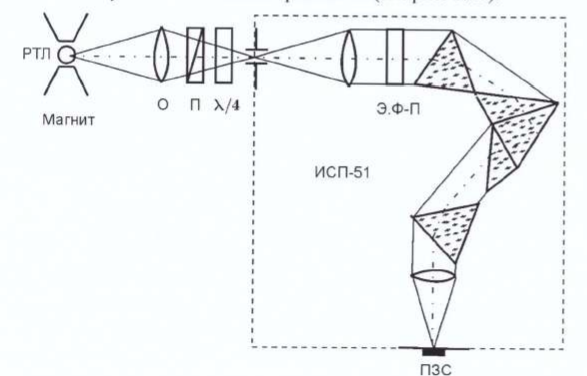
\includegraphics[width=1\linewidth]{ust}
		\caption{Экспериментальная установка}
	\end{figure}
	В работе исследуется расщепление линий ртути в магнитном поле. Источником излучения является ртутная лампа, спектр которой представляет собой набор достаточно далеко отстоящих друг от друга отдельных линий.
	Область дисперсии изучаемого в работе ЭФП составляет
	$\Delta \lambda \sim 0.2-0.3 \mathrm{~A}$ для видимой области спектра. Она существенно меньше расстояния между отдельными линиями излучения ртути. По этой причине необходима предварительная монохроматизация излучения. В нашей работе применена стандартная схема предварительной монохроматизации, в которой используется призменный спектрограф ИСП-51.
	
	Возможны два варианта установки эталона относительно спектрографа: перед входной щелью прибора или внутри его.
	
	Так как эталон работает в параллельном пучке лучей, то при установке перед щелью необходимо использование дополнительных объективов и тщательная юстировка оптической схемы.
	
	Установка эталона внутри спектрографа более удобна в работе, хотя при этом наблюдается увеличение количества рассеянного света. Этот вариант используется в наших экспериментах
	Линии ртутной лампы в фокальной плоскости камерного объектива спектрографа пространственно разделены в горизонтальном направлении за счет дисперсии призменного спектрографа ИСП-51. Их изображения при достаточно узких щелях не накладываются друг на друга. При этом в изображении каждой линии в вертикальном направлении из-за дисперсии эталона Фабри-Перо видны части интерференционных колец, которые в горизонтальном направлении ограничены размером входной щели. В случае такого расположения двух спектральных приборов с перпендикулярными направлениями дисперсии говорят об их "скрещенной" установке.
	
	Наблюдение расщепления линий в магнитном поле проводится в вертикальной плоскости, т.е. в направлении дисперсии эталона Фабри-Перо.
	
	Свет от ртутной лампы РТЛ, помещенной между полюсами электромагнита, с помощью конденсора O проектируется на входную щель спектрографа. Электромагнит установлен на поворотном столике. Это позволяет наблодать эффект Зеемана в поперечном и продольном полях.
	
	Регистрация спектра осуществляется с помощью видеокамеры на основе ПЗС-матрицы. Полученная картина отображается на видеомониторе или экране компьютера.
	
	Для поляризационных измерений используются поляризатор П и пластинка $\lambda / 4$.
	\\
	Максимальный порядок интерференции при нормальном падении света на ЭФП через $m_0$, порядок интерференции, в котором производим измерение через $m$.
	Тогда, в $m$-м порядке
	для длины волны $\lambda_0$ угловые размеры кольца $\varphi_{\text {h }}$ определяются соотношениями
	$$
	\begin{aligned}
		& m \lambda=2 t \sqrt{n^2-\sin ^2\left(\phi_h\right)}, \\
		& \phi_h=\arcsin \left[n \sqrt{\left(1-\left(\frac{m}{m_0}\right)^2\right)}\right]
	\end{aligned}
	$$
	
	для длины волны расщепления Зеемана $\lambda=\lambda_0 \pm \delta \lambda$ угловые размеры кольца $\varphi_{\text {mid }}$ определяются выражением
	$$
	m(\lambda+\delta \lambda)=2 t \sqrt{n^2-\sin ^2\left(\phi_{\operatorname{mid}}\right)} ;
	$$
	
	для длины волны $\lambda_0 \pm \Delta \lambda$, где $\Delta \lambda$ - область дисперсии, угловые размеры кольца  могут быть записаны как
	$$
	\begin{aligned}
		& m(\lambda+\Delta \lambda)=2 t \sqrt{n^2-\sin ^2\left(\phi_1\right)}, \\
		& \phi_1=\arcsin \left(\sqrt[n]{\left(1-\left(\frac{m}{m_0}\left(1+\frac{\Delta \lambda}{\lambda_0}\right)\right)^2\right)} .\right.
	\end{aligned}
	$$
	Переходя к радиусам колец, получаем $r_{\mathrm{h}}-r_{\text {mid }}=F\left(\varphi_{\mathrm{h}}-\varphi_{\text {mid }}\right)$ и $r_{\mathrm{h}}-n_1=F\left(\varphi_{\mathrm{h}}-\varphi_1\right)$.
	Обозначая через Q отношение разности радиусов колец
	$$
	\mathrm{Q}=\frac{r_h-r_i}{r_{\text {mid }}-r_j}=\frac{\phi_h-\phi_{\text {mid }}}{\phi_h-\phi_l},
	$$
	
	находим
	$$
	\phi_{\text {mid }}=Q \phi_l+(1-Q) \phi_h .
	$$
	
	Величины $\varphi_{\mathrm{h}}$ и $\varphi_1$ вычисляются по параметрам эталона, после чего из соотношений (5.5) и (5.3) находим значение $\varphi_{\text {mid }}$ и величину расщепления Зеемана:
	$$
	\delta \lambda=\lambda\left(\frac{m_0}{m}-1\right) \sqrt{1-\frac{1}{n^2} \sin \left(\phi_{\text {mid }}\right)} .
	$$
	
	\begin{enumerate}
		\item По пикам полученными на распределении интенсивности определим величину Q:
		
		$$ Q = \frac{|108-215|}{|108-334|} = 0,47 $$
		
		\item Рассчитаем значения $\phi_h$ и $\phi_l$:
		
		$$ \phi_h=\arcsin \left[n \sqrt{\left(1-\left(\frac{m}{m_0}\right)^2\right)}\right] = 0,02690 \text{рад}$$
		
		$$ \phi_1=\arcsin \left(\sqrt[n]{\left(1-\left(\frac{m}{m_0}\left(1+\frac{\Delta \lambda}{\lambda_0}\right)\right)^2\right)} .\right. = 0,02400 \text{рад}$$ 
		
		\item Тогда посчитаем $\delta \lambda$:
		
		$$ \delta \lambda=\lambda\left(\frac{m_0}{m}-1\right) \sqrt{1-\frac{1}{n^2} \sin \left(\phi_{\text {mid }}\right)} = 0,06 \text{\AA} $$
		
		\item Посчитаем поле:
		
		$$ B_{\text{теор}} = \frac{4\pi c^2 m}{ e \lambda^2} \delta \lambda = 38 \text{Тл}$$
		
		$$ B_{\text{эксп}} = 55 \text{Тл, т.к. расщепление $\delta \lambda $= 0,088 \AA}$$
		
		
		\begin{figure}[h!]
			\centering
			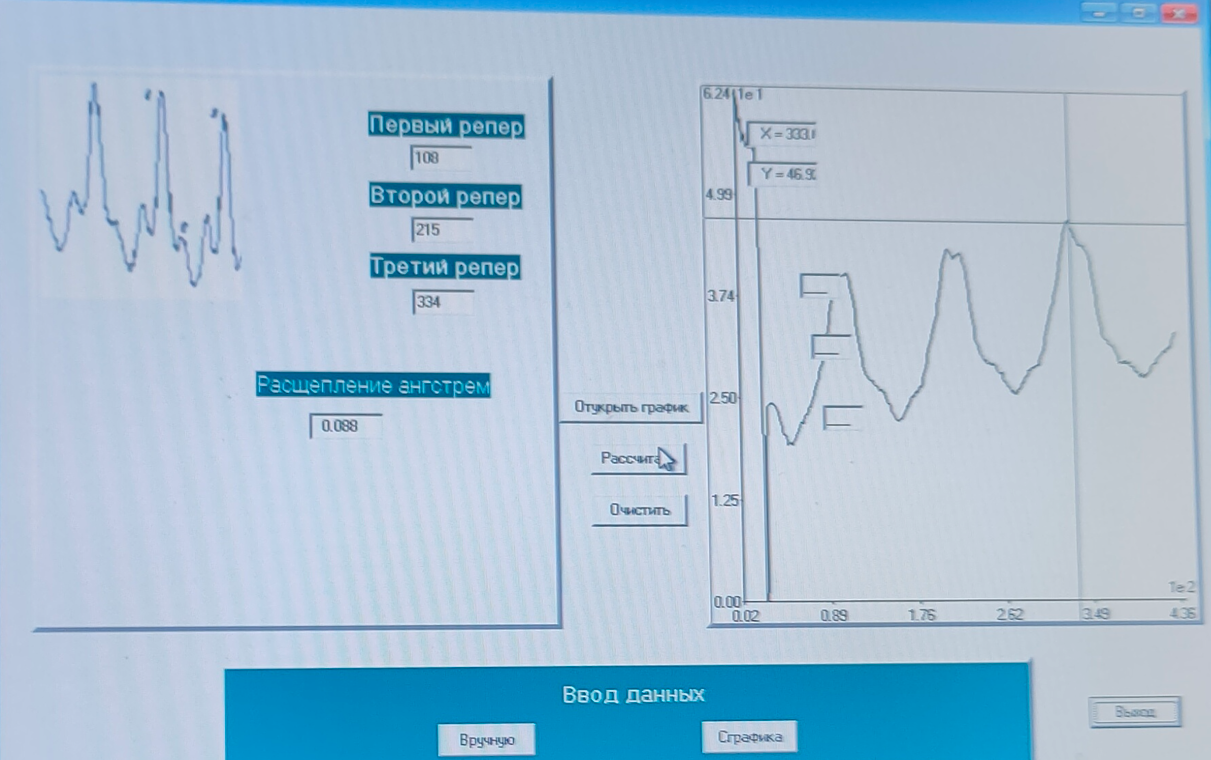
\includegraphics[width=1\linewidth]{graph}
			\caption{Полученный график в ПО на ЭВМ}
		\end{figure}
		
		
		
		
	\end{enumerate}
	
	\textbf{Обсуждение результатов и выводы: }\\
	
	В ходе работы мы изучили принцип работы интерферометра Фапри-Перо, наблюдали эффект Зеемана. Также определили величину поля магнита.
	
	
	
	
	
	
	
	\end{document}